\section{Methods}\label{sec:methods}

\subsection{Genome-Scale Models}\label{ssec:genome_scale_models}

% \begin{itemize}
%  \item How are they created?
%  \begin{itemize}
%   \item genome or annotated genome are automatically translated to a GEM
%   \item tools: Pathway Tools \cite{karp2009pathway}, SEED \cite{henry2010high}
%   \item AUTOGRAPH \cite{notebaart2006accelerating} which reuses existing models
%   \item \cite{santos_practical_2011}
%   \item must be refined by hand
%   \item ``too many important organism-specific choices''
%   \item ``omissions, wrong assignments and gaps, and inconsistencies''
%   \item biomass function
%   \item input/output reactions
%   \item ``gene-to-protein-to-reaction (GPR) association that describes the genetic basis for a
% metabolic reaction ''
%   \item A reconstruction collects all the available
% biochemical, genetic, and genomic (BiGG) information that is available on a cellular
% process of interest, and then organizes it in a formal, mathematical fashion that is
% consistent with the corresponding fundamental chemical and genetic properties
%   \item \cite{palsson2015systems}
%   \item Networks are composed of compounds (nodes) and reactions (links)
%   \item Such mathematical
% representation is based on the stoichiometric coefficients that count the molecules that
% are consumed and produced by a biochemical reaction.
%   \item It is important to note that a map for a network can be drawn in many
% different ways, but the mathematical representation is unique.
%   \item Ultimately, a reconstruction can reach a genome-scale when all the known
% biochemical and genetic processes that are found on a genome are accounted for
%   \item they now include the details of both protein
% synthesis and structure, transcriptional regulation, and other processes
%   \item A network reconstruc-
% tion is the basis for a computational model for network states (i.e., phenotypic states)
%  \end{itemize}
% 
%  \item What does they contain?
%  \item What is missing?
% \end{itemize}

A genome-scale model (GEM) is an analytical reconstruction of ideally all cellular process of a cell.
All available biochemical, genetic and genomic (BiGG) information of the processes are analyzed to
identify gene-to-protein-to-reaction (GPR) associations and involved compounds. 
Based on this data a network composed of compounds (nodes) and reactions (links) is created and added
to the reconstruction.
\cite{palsson2015systems}

Tools like \textit{Pathway Tools}\cite{karp2009pathway},
\textit{SEED}\cite{henry2010high} or \textit{AUTOGRAPH}\cite{notebaart2006accelerating} are used to
generate a reconstruction based on a (annotated) genome. The produced models contain many
wrong assignments, gaps and inconsistencies due to many organism-specific choices and must be refined by hand.
A biomass function to model growth and input/output reactions are added to
the network\cite{santos_practical_2011}.

The reconstruction is the basis for mathematical models and further analysis.
One important mathematical representation is the stoichiometric matrix. It uniquely represents the metabolic
network of the cell, based on the stoichiometric constants of its reactions\cite{palsson2015systems}.


\begin{figure}[!h]
\centering
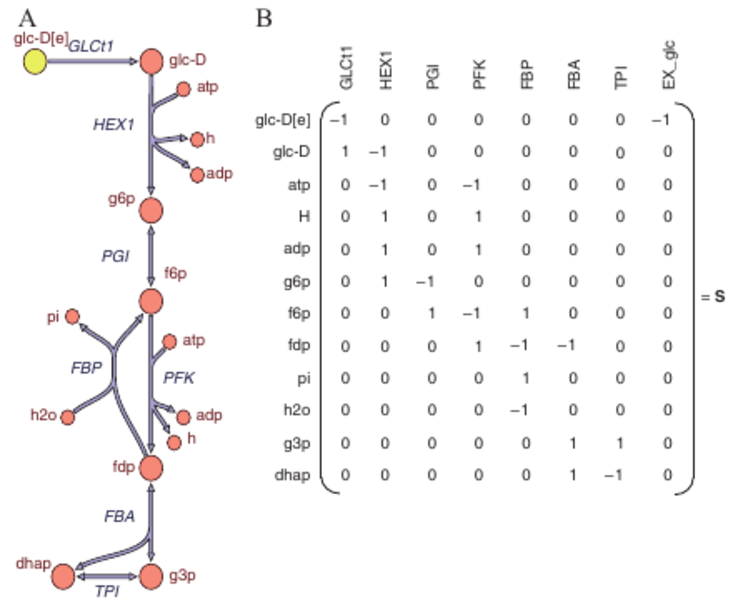
\includegraphics[width=\linewidth]{figures/Selection_011.pdf}
\caption{(create simplified version here, combine with figure \ref{fig:reconstruction_GPR_example})}
\label{fig:reconstruction_to_matrix_example}
\end{figure}

\begin{figure}[!h]
\centering
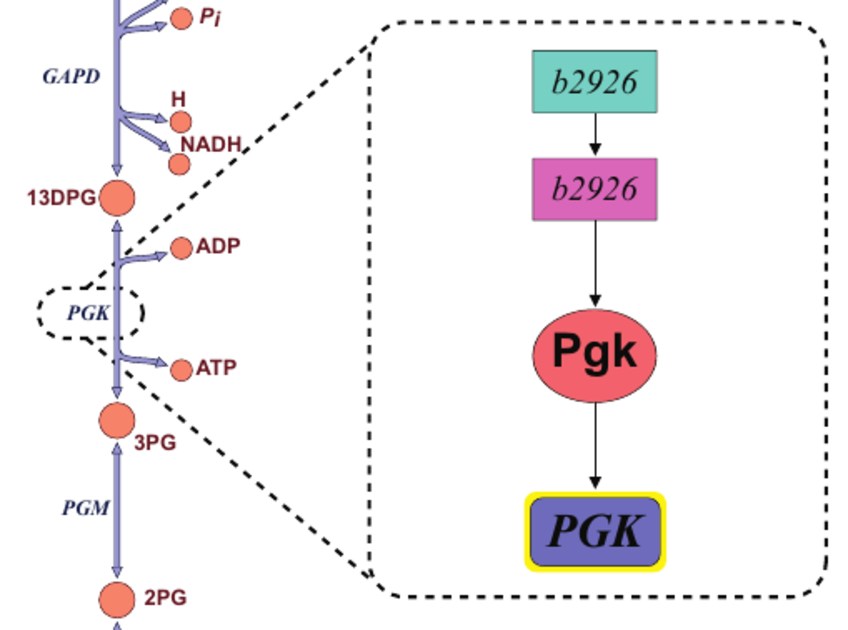
\includegraphics[width=\linewidth]{figures/Selection_013.pdf}
\caption{(create simplified version here, combine with figure \ref{fig:reconstruction_to_matrix_example})}
\label{fig:reconstruction_GPR_example}
\end{figure}

\subsection{Flux Balance Analysis}\label{ssec:flux_balance_analysis}

\cite{orth_what_2010}



\subsection{Simulation Algorithm}

\begin{table}[h]
\centering
\caption{Overview of implemented features compared to DMMM}
\label{tab:overview_implemented_features_compared_to_dmmm}
\begin{tabular}{llllll}
\rowcolor[HTML]{EFEFEF} 
\cellcolor[HTML]{EFEFEF} Feature                  & \cellcolor[HTML]{EFEFEF}DMMM & \cellcolor[HTML]{EFEFEF}This project\\
Model                                    &   &  \\
\hspace{0.5cm}arbitrary many GEMs & yes & yes \\
\hspace{0.5cm}\begin{tabular}[c]{@{}l@{}}arbitrary many metabolites\\ in environment\end{tabular} & yes & yes \\
\hspace{0.5cm}mortablility of bacteria & \begin{tabular}[c]{@{}l@{}}yes\\(in output flux)\end{tabular} & yes \\
\hspace{0.5cm}\begin{tabular}[c]{@{}l@{}}input/output flux of bacteria\\ and metabolites\end{tabular} & yes & no \\
\hspace{0.5cm}\begin{tabular}[c]{@{}l@{}}parameterized initial state\\ of environment composition\end{tabular} & yes & yes \\
\hspace{0.5cm}Michaelis-Menten kinetics & yes & yes \\
Algorithm &  &  \\
\hspace{0.5cm}ODE solver & yes & yes \\
\hspace{0.5cm}different ODE solvers & yes & no \\
\hspace{0.5cm}analytical solver & yes &no \\
\end{tabular}
\end{table}

As described by Zhuang et al. in \cite{zhuang_genome-scale_2011} the algorithm uses a ODE solver with embedded FBA. A FBA is solved
for each GEM in the model and for each time step in the discretised simulation time interval considering the changed metabolite and
bacteria densities in the shared environment. The results of the FBAs are used by the ODE solver to solve the differential equations

\begin{equation} \label{eq:diff_eq_x}
 \frac{\mathrm d x_j}{\mathrm d t} = \mu_j x_j
\end{equation}
\begin{equation} \label{eq:diff_eq_s}
 \frac{\mathrm d s_i}{\mathrm d t} = \displaystyle\sum_{j=1}^{N} v_{i,j} x_j
\end{equation}

which models the dynamics of the bacteria's environment \cite{zhuang_design_2012} where $i = 1...N$ is the index of metabolites in the shared environment and $j = 1...M$ is the index of bacteria.
The bacteria density is modeled in $x_j$ with $\left[ x_j \right] = \si{\gram}$ and $\mu_j$ is the bacteria's growth rate with $[\mu_j] = \si{\gram\per\gram_{DW}\per\hour}$.
Input and output fluxes of the bacteria's models are modeled in $v_{i,j}$ with $\left[ v_{i,j} \right] = \si{\milli\mole\per\gram_{DW}\per\hour}$,
the densities of metabolites in the shared environment in $s_i$ with $\left[ s_i \right] = \si{\milli\mole\per\liter}$.

In each time step each bacteria's metabolite intake must be changed dependent on the densities of the metabolites in the shared environment.
To model saturation of metabolite intake for high metabolite densities Zhuang et al. implemented Michaelis-Menten kinetics \cite{johnson2011original}

\begin{equation} \label{eq:michaelis-menten}
 v_{max,i,j} = \frac{v_{mm,i,j} s_i}{s_i + k_{mm,i,j}} \frac{1}{1 + \frac{s_a}{k_{a,i,j}}}
\end{equation}

This formula describes the upper bound of the input flux $v_{max,i,j}$ for metabolite i of bacteria j dependent on the metabolite density
$s_i$. The formula is characterized by to constants $\left[ v_{mm,i,j} \right] = \si{\milli\mole\per\gram_{DW}\per\hour}$ and $\left[ k_{mm,i,j} \right] = \si{\milli\mole\per\liter}$
for each bacteria and metabolite. $s_a$ is the metabolite density of metabolite a, $k_{a,i,j}$ is the inhibition constant of metabolite a and
describes the inhibition of the intake of metabolite i by metabolite a at species j.

Mortality is considered using a constant $\left[ \mu_{mort,j} \right] = \si{\milli\mole\per\gram_{DW}\per\hour}$ for each bacteria j in this implementation while Zhuang et al. modeled this
using the output flux of bacteria out of the system.

Algorithm \ref{alg:differential_equation_with_embedded_fba} shows a basic implementation of the differential equations solved by an ODE
solver during the simulation similar to DMMM \cite{zhuang_genome-scale_2011}.

The algorithm expects a list of bacteria models consisting of
\begin{itemize}
 \item GEM of this bacteria: A, $\bm{v_{min}}$, $\bm{v_{max}}$, $\bm{w_{growth}}$
 \item $\bm{v_{mm}}$ (Michaelis-Menten $V_{max}$) for each exchange metabolite and species
 \item $\bm{k_{mm}}$ (Michaelis-Menten K) for each exchange metabolite and species
 \item mortality $\mu_{mort}$
 \item inhibition constants $k_a$
\end{itemize}

Furthermore a list of all exchange metabolites in the environment, the bacteria and metabolite densities.


\begin{algorithm}
    %\SetKwInOut{Input}{Input}
    %\SetKwInOut{Output}{Output}

%    \underline{derivative}$(model_1...model_M, m_1...m_N, x_1...M, s_1...s_N)$\;
	\def\model{\ensuremath{\mathrm{model}}}
    \KwIn{bacteria populations $x_j$, metabolite counts $S_i$}
    \KwOut{slope of bacteria and metabolite densities $\dot{x}_j, \dot{s}_i$}
    \KwData{bacteria models $\model_j$, Michaelis-Menten constants of model $M$ $\v{k}_{M}$, inhibition matrices of model $M$  $\mat{I}_{M}$}
    \def\lb{\mathrm{lb}}
    
    $s_i \KwAssign \frac{S_i}{V}$\;
    
    $S_{<0} \KwAssign \{m | S_m < 0\}$\;
    $x_{<0} \KwAssign \{j | x_j < 0\}$\;

    
	$\v s(S_{<0}) = 0$\;
	$\v x(S_{<0}) = 0$\;
	
	\ForEach{model $M$ in models}{
		\ForEach{metabolite $m$ in exchanges of $M$}{
			$\displaystyle \lb_{M,m} = \lb_{M,m,ini} \; \frac{s_m}{k_{M,m}+s_m} \; \prod_{m'} \cfrac{1}{1+\cfrac{s_{m'}}{\mat{I}_{M,m,m'}}}$\;
		}
	}
	
	$\dot{\v x} \KwAssign [0,\dotsc,0]$\;
	$\dot{\v S} \KwAssign [0,\dotsc,0]$\;
	
    \ForEach{Model $M$ in models}{
      $\mu, \bm{v}$ \KwAssign FBA($M$)\;
      $\dot{x}_M = \mu \mul x_M$\;
      $\dot{\v S} = \dot{\v S} + \v v \mul x_M$\;
    }
    
	$\dot{\v S}(S_{<0}) = \max\{0,\dot{\v S}(S_{<0})\}$\;    
	$\dot{\v x}(x_{<0}) = \max\{0,\dot{\v x}(x_{<0})\}$\;    
    
    \Return{$[\dot{\v x},\dot{\v S}]$}
    \caption{Differential equation with embedded FBA}
    \label{alg:differential_equation_with_embedded_fba}
\end{algorithm}

In a first step the upper bounds of the intake fluxes are updated for each bacteria j and exchange metabolite i.
The function $update\_intake\_bounds(model_j, s_j, m_i)$ calculates the upper bounds using the formula \ref{eq:michaelis-menten} if
the metabolite $m_i$ is contained in $model_j$ as a exchange metabolite and updates this value in the model.

In a next step the GEMs are optimized for growth using FBA, the results are used as growth rate $\mu_j$ and actual input and output
fluxes $\bm{v_j}$ of bacteria j in this time step.

The mortality is considered by subtracting the constants $\bm{\mu}$ from the growth rates $\bm{\mu}$.

At last step the slopes $\dot{\bm{x}}$ and $\bm{\dot{s}}$ are calculated according to \ref{eq:diff_eq_x} and \ref{eq:diff_eq_s} and
returned to the ODE solver.


\subsection{Simulation Setup}\label{ssec:simulation_setup}

The goal of the simulation is to validate the basic functionality of the simulator using a simplified setup of a realistic future
simulation scenario. As defined in our project goals, this simulation scenario is the dynamic flux balance analysis (DFBA) of a
co-culture of Saccharomyces cerevisiae and Lactobacillus plantarum.

As genome-scale models a model of Lactobacillus plantarum published by Teusink et al. \cite{teusink_analysis_2006}. A decision about
a yeast model is not made yet.

The simulation will consider two input metabolites: oxygen and glucose. Table \ref{tab:model_constants_simulation_setup} and table
\ref{tab:simulation_parameters_simulation_setup} contain all values needed to define the initial metabolite conditions and kinetics.

\begin{table}[h]
\centering
\caption{Model constants used in the simulation setup}
\label{tab:model_constants_simulation_setup}
\begin{tabular}{llllll}
\rowcolor[HTML]{EFEFEF} 
\cellcolor[HTML]{EFEFEF} Constant          & \cellcolor[HTML]{EFEFEF}S. cerevisiae & \cellcolor[HTML]{EFEFEF}L. plantarum\\
Maximum glucose uptake rate (mmol/g/h)     & 18.5 & 18.5 \\
Maximum oxygen uptake rate (mmol/g/h)      & 2.5 & 2.5 \\
Glucose uptake saturation constant (g/l)   & 0.5 & 0.5 \\
Oxygen uptake saturation constant (mmol/l)     & 0.005 & 0.005 \\
Mortability (?)                            & ? & ? \\
Glucose uptake inhibition by ethanol constant (g/l)     & 10\cite{hjersted_genome-scale_2007} & - \\
Glucose uptake inhibition by lactic acid constant (mol/mol ?)     & TBD & - \\
\end{tabular}
\end{table}

% E-Mail from Steinn about model constants of L. plantarum from 12.04.2018:
% ----------------------------------------------------------------------------------------------
% As a first approximation I would assume the same v_max and k_m for L. plantarum as in yeast.
% 
% The maximum glucose uptake rate can be assumed to be similar to yeast for the time being 
% (for Lactobacillus reuteri it is approx. 21 mmol/gDW/h [gDW = grams dry weight]). L. plantarum 
% is an anaerobe that can tolerate oxygen (and has some oxygen dependent metabolism as well) but
% as a first approximation I would assume that oxygen plays a minor role, hence the oxygen
% saturation constant may not be too important.
% ----------------------------------------------------------------------------------------------

\begin{table}[h]
\centering
\caption{Simulation parameters used in the simulation setup}
\label{tab:simulation_parameters_simulation_setup}
\begin{tabular}{llllll}
\rowcolor[HTML]{EFEFEF} 
\cellcolor[HTML]{EFEFEF} Parameter          & \cellcolor[HTML]{EFEFEF}value & \cellcolor[HTML]{EFEFEF}reference\\
Initial glucose density (mmol/l) & 272.9 ... 1230.755 & equation \ref{eq:ready_to_use_plato_to_metabolite_density}, table \ref{tab:constants_used_in_this_document} \\
Initial oxygen density (mmol/l)  & 0.5039 & equation \ref{eq:init_oxygen_density}, table \ref{tab:constants_used_in_this_document}\\
Initial density of S. cerevisiae (mmol/l) & ? & - \\
Initial density of L. plantarum (mmol/l) & ? & - \\
\end{tabular}
\end{table}

To verify the basic functionality of the simulator the resulting bacteria densities and metabolite densities of ethanol, d- and l-lactate,
oxygen and glucose will be compared to existing data.
